\section{Analysis}\label{sec:analysis}
\subsection{Sensitivity to costs, constraints and timing}
In Table~\ref{tab:robustness}, the sentiment-driven portfolio's Sharpe ratio stays above equal weighting with a lower entry band of 1~s.d. (\RobEntryBandOneSDSentimentSharpe), with a one- or four-week half-life, and when news reaches the portfolio one session later (\RobNewsOneSessionLaterSentimentSharpe). The higher 2~s.d. band and the 10\% position limit leave it slightly below.

The cost results are not monotonic (Figure~\ref{fig:costs}). The sentiment-driven portfolio has a higher Sharpe ratio than equal weighting at every cost level, and without costs it earns \RobCostsZeroBpPerTradeSentimentCAGR{} a year against \RobCostsZeroBpPerTradeEWCAGR{}. At 20 bp all optimisers trade less, and the price-only portfolio performs best of all. A different cost rate changes the trades the optimiser makes as well as the net return, and the spread across scenarios is as large as the differences between strategies.
\end{multicols}
\begin{table}[H]\centering\footnotesize\setlength{\tabcolsep}{4pt}\begin{tabular}{lccccc}
\toprule
Scenario & Sentiment-driven & Price + sentiment & Price only & Minimum variance & Equal weight \\
\midrule
Base case & 11.90 / 0.64 & 12.20 / 0.65 & 10.28 / 0.54 & 9.41 / 0.60 & 12.15 / 0.63 \\
Costs 20 bp per trade & 12.99 / 0.70 & 12.72 / 0.70 & 13.74 / 0.75 & 10.41 / 0.66 & 12.00 / 0.62 \\
Position limit 10\% & 11.73 / 0.62 & 12.05 / 0.64 & 10.67 / 0.56 & 8.80 / 0.56 & 12.15 / 0.63 \\
Entry band 1 s.d. & 12.57 / 0.67 & -- & -- & -- & -- \\
Entry band 2 s.d. & 11.48 / 0.61 & -- & -- & -- & -- \\
Gauge half-life 1 week & 12.70 / 0.68 & 12.30 / 0.65 & -- & -- & -- \\
Gauge half-life 4 weeks & 12.13 / 0.65 & 13.02 / 0.70 & -- & -- & -- \\
News one session later & 12.29 / 0.66 & 12.40 / 0.65 & -- & -- & -- \\
2015-2019 & 8.79 / 0.62 & 8.94 / 0.62 & 6.84 / 0.50 & 10.87 / 0.93 & 9.20 / 0.65 \\
2020-2025 & 14.57 / 0.66 & 15.01 / 0.68 & 13.25 / 0.59 & 8.21 / 0.42 & 14.67 / 0.64 \\
\bottomrule
\end{tabular}

\caption{Robustness: CAGR (\%) / Sharpe ratio after costs. One setting is changed at a time; ``--'' means the strategy is unaffected. Costs of 0 and 5 bp are shown in Figure~\ref{fig:costs}.}\label{tab:robustness}\end{table}
\begin{figure}[H]\centering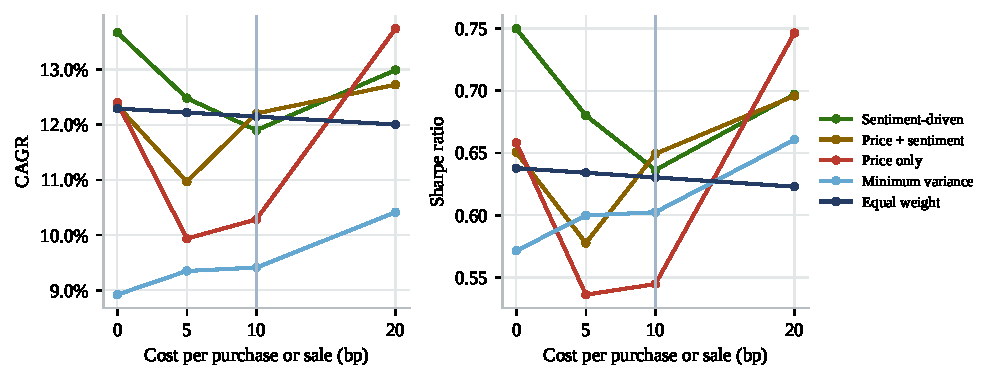
\includegraphics[width=\textwidth]{costs}
\caption{Net CAGR and Sharpe ratio as functions of the cost per purchase or sale. The vertical line marks the base case.}\label{fig:costs}\end{figure}
\begin{multicols}{2}

\subsection{Market conditions and sources of return}
In 2015--2019 minimum variance had the highest Sharpe ratio (\RobTwoZeroOneFiveTwoZeroOneNineMinVarSharpe) and the sentiment-driven portfolio trailed equal weighting slightly; in 2020--2025 the sentiment-driven and price + sentiment portfolios had the highest Sharpe ratios (\RobTwoZeroTwoZeroTwoZeroTwoFiveSentimentSharpe{} and \RobTwoZeroTwoZeroTwoZeroTwoFiveCombinedSharpe). Relative to equal weighting, the sentiment-driven portfolio returned \UpSentimentEW{} basis points a week in rising markets and \DownSentimentEW{} in falling markets (both insignificant), which suggests that its smaller drawdown comes from defensive behaviour in sell-offs.

On average the sentiment-driven portfolio held about 8 percentage points more information technology and 7 points less financials than equal weighting (Figure~\ref{fig:tilts}). Technology outperformed during the test period, so part of the result may come from this sector tilt rather than from picking stocks within sectors.
\end{multicols}
\begin{figure}[H]\centering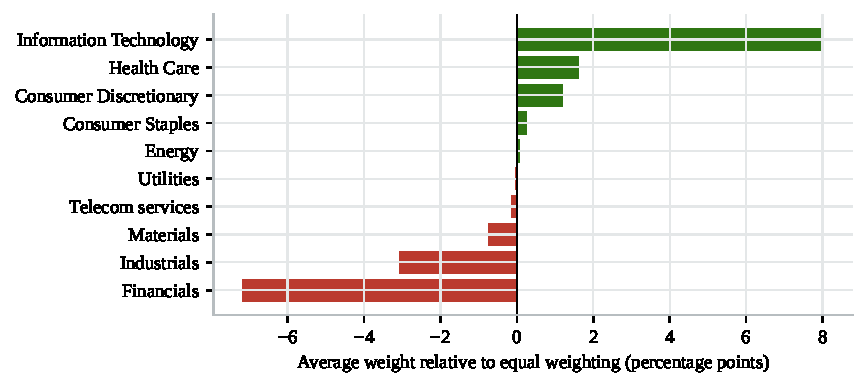
\includegraphics[width=0.8\textwidth]{sector_tilts}
\caption{Average sector weight of the sentiment-driven portfolio relative to equal weighting, 2015--2025.}\label{fig:tilts}\end{figure}
\begin{multicols}{2}
